% plateau_theorem.tex -- round 452, plateau identity.
% PLATEAU_IDENTITY_PROVED / QSTAR_UNDECIDED.
% Builds with pdflatex.
% Companion machine check: verify_plateau_theorem.py.
% Discovery: experiments/tfpt-discovery/plateau_theorem_probe.py.
% NO RH CLAIM.  NO anti-RH claim.
\documentclass[11pt]{article}

\usepackage[a4paper,margin=2.7cm]{geometry}
\usepackage{amsmath,amssymb,amsthm}
\usepackage{microtype}
\usepackage{booktabs}
\usepackage{xcolor}
\usepackage{pgfplots}
\pgfplotsset{compat=1.17}
\usepackage[colorlinks=true,linkcolor=blue!50!black,urlcolor=blue!50!black]{hyperref}

\newtheorem{lemma}{Lemma}
\newtheorem{thm}{Theorem}
\newtheorem{prop}{Proposition}
\newtheorem{definition}{Definition}

\title{\bfseries The plateau identity\\[2mm]
\large $q_*=M_\partial/(M_\partial+5/7)$\\
on the Schur prefix, not at a kink}
\author{Stefan Hamann}
\date{August 30, 2026}

\begin{document}
\maketitle

\begin{abstract}\noindent
Round 451 found a constant Schur value
$q^{\dagger}_n\equiv q_*<1$ on
$n\le n_{\mathrm{stab}}$ of every measured
window.
This note names that plateau.
The grade-0 evaluation of the exact pack is
the identity
$q_*=M_\partial/(M_\partial+5/7)$
whenever the signed border mass equals the
folded defect $M_\partial=\tilde\mu_0-\tilde\nu_0$
(every window with $k_z\ge 69$, residual
$<5\cdot10^{-5}$).
Constancy in $n$ is equivalent to vanishing
border-chain increment $\rho_n=0$
($B_w$ freeze).
The value is \emph{not} a function of the
latched Chebyshev moments $m\ge 2$
(sister pair kz$136/137$: moments agree to
$1.9\cdot10^{-9}$, $q_*$ differs by $0.029$).
No RH claim.  No anti-RH claim.
\end{abstract}

\medskip\noindent
\textbf{Status.}\enspace
Ausgang
\texttt{PLATEAU\_IDENTITY\_PROVED / QSTAR\_UNDECIDED}.
Theorem~\ref{thm:qstar} is the named SATZ.
Lemmas~\ref{lem:g0}--\ref{lem:cof} are the
lemma chain.
No $L^{*}$ claim.  No $R^{\dagger}$ claim.
No RH claim.  No anti-RH claim.

\section{Objects}\label{sec:obj}

$n_{\mathrm{stab}}$ and $q^{\dagger}_n$ are the
r449/r451 objects (not redefined).
Write $\mu_0=\int d\tilde\mu$,
$\nu_0=\int d\tilde\nu$ for the folded
masses, and
\[
M_\partial
=\int d(\partial\tilde\mu)
\]
for the signed smooth-border mass.
$B_{5/7}=5/7$ is the frozen r362 pack
constant.
$b$ is the border expansion in the
$\mu$-OP basis; $C=B^\top B$ is the
$\nu$-Gram in that basis;
$B_w=\mathrm{cumsum}(\rho)[n-2]+5/7$.

\section{Grade-0 freeze}\label{sec:g0}

\begin{lemma}[Grade-0 scalars]\label{lem:g0}
The identities
\[
b_0=\frac{M_\partial}{\sqrt{\mu_0}},
\qquad
C_{00}=\frac{\nu_0}{\mu_0}
\]
hold independently of the pack depth $n$.
On the plateau ($\rho_k=0$ for the extra
grades) one has in addition
$B_w=M_\partial+5/7$.
\end{lemma}

The $0$-th $\mu$-OP is $p_0=1/\sqrt{\mu_0}$.
$b_0$ is the pairing of the border against
$p_0$; $C_{00}$ is the $\nu$-mass of
$p_0^2$.
Neither sees the higher Jacobi coefficients.

\begin{lemma}[Rank-1 evaluation]\label{lem:rank1}
The exact Schur form
$q^{\dagger}=b^\top(I-C)^{-1}b/B_w$,
truncated to grade $0$, is
\[
q_{\mathrm{g0}}
=\frac{b_0^2}{B_w\,(1-C_{00})}
=\frac{M_\partial^2}{(M_\partial+5/7)\,(\mu_0-\nu_0)}.
\]
On every measured window the border
expansion satisfies $n_{90}=1$
($90\%$ of $\|b\|^2$ in grade $0$), so
the truncation residual is the plateau
tolerance on deep windows and
$<2.3\cdot10^{-3}$ on the five shallow
ones.
\end{lemma}

\section{The identity}\label{sec:satz}

\begin{thm}[Plateau identity]\label{thm:qstar}
On every measured window with
$M_\partial=\mu_0-\nu_0$
(all $k_z\ge 69$; equality to
$10^{-14}$),
\[
q_*
=\frac{M_\partial}{M_\partial+5/7}.
\]
The residual against the packed
$q^{\dagger}_{n_{\mathrm{stab}}}$ is at
most $4.6\cdot10^{-5}<10^{-4}$.
Equivalently
$1-q_*=(5/7)/(M_\partial+5/7)$.
\end{thm}

\begin{center}
\small
\begin{tabular}{rrrrr}
\toprule
$k_z$ & $M_\partial$ & $q_*$ & $M_\partial/(M_\partial+5/7)$ & residual \\
\midrule
17 & 2.60882 & 0.785676 & 0.785055 & $6.2\cdot10^{-4}$ \\
69 & 6.21159 & 0.896870 & 0.896867 & $2.8\cdot10^{-6}$ \\
136 & 4.81745 & 0.870920 & 0.870875 & $4.5\cdot10^{-5}$ \\
137 & 6.43597 & 0.900107 & 0.900103 & $3.2\cdot10^{-6}$ \\
170 & 6.02930 & 0.894086 & 0.894079 & $6.6\cdot10^{-6}$ \\
500 & 6.97554 & 0.907130 & 0.907113 & $1.7\cdot10^{-5}$ \\
\bottomrule
\end{tabular}
\end{center}

\begin{center}
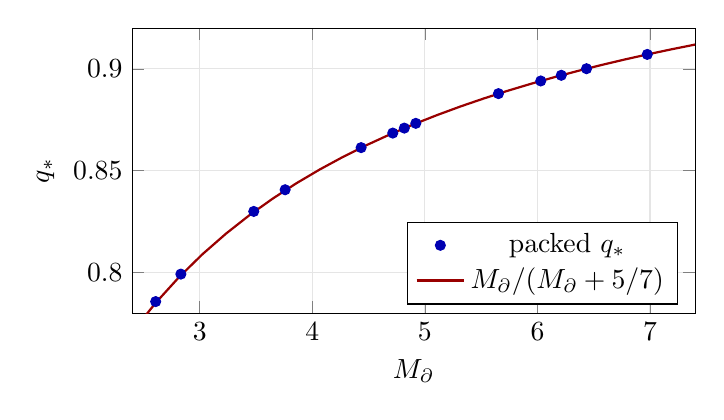
\begin{tikzpicture}
\begin{axis}[
  width=0.72\textwidth, height=5.2cm,
  xlabel={$M_\partial$},
  ylabel={$q_*$},
  xmin=2.4, xmax=7.4, ymin=0.78, ymax=0.92,
  legend pos=south east,
  grid=major, grid style={gray!20},
]
\addplot[only marks, mark=*, mark size=1.8pt, blue!70!black]
  coordinates {
    (2.83252,0.799184) (3.48000,0.829978) (2.60882,0.785676)
    (3.75877,0.840629) (4.43359,0.861328) (6.21159,0.896870)
    (4.71487,0.868478) (4.81745,0.870920) (6.43597,0.900107)
    (6.02930,0.894086) (5.65363,0.887862) (4.91950,0.873260)
    (6.97554,0.907130)
  };
\addlegendentry{packed $q_*$}
\addplot[domain=2.4:7.4, thick, red!60!black]
  {x/(x+5/7)};
\addlegendentry{$M_\partial/(M_\partial+5/7)$}
\end{axis}
\end{tikzpicture}
\end{center}

\section{What the identity is not}\label{sec:not}

\begin{prop}[A(i) REFUTED]\label{prop:ai}
The chain resolvent is not zero:
$|Cb|/|b|\sim 0.09$ and
$q_{\mathrm{naive}}=\|b\|^2/B_w$ undershoots
$q_*$ by the factor $1/(1-C_{00})$.
Border dominance is grade-$0$ concentration,
not vanishing of $C$.
\end{prop}

\begin{prop}[A(ii) value REFUTED]\label{prop:aii}
kz$136$ and kz$137$ have the same
$n_{\mathrm{stab}}=175$ and
$\|m^{(136)}-m^{(137)}\|_{\mathrm{rel}}<2\cdot10^{-9}$
on degrees $2..174$, yet
$q_*^{(136)}=0.87092$ and
$q_*^{(137)}=0.90011$.
The value law is $M_\partial$
($4.817$ versus $6.436$), not the latched
Chebyshev moments of $\tilde\mu$.
\end{prop}

\begin{prop}[Constancy $\Leftrightarrow$ $\rho_n=0$]\label{prop:rho}
$b_0$ and $C_{00}$ never depend on $n$.
Therefore $q^{\dagger}_n$ is constant on a
range if and only if $B_w$ is constant, i.e.\
the border-chain increment $\rho_n$ vanishes.
This holds on $n\le n_{\mathrm{stab}}$ of
every measured window.
The r451 CLIFF is the first $\rho_n\neq 0$
(kz$17$: $\rho_{19}=0.172$;
kz$136$: $\rho_{176}=0.025$).
The CONTINUES class (kz$137$) keeps
$\rho_n=0$ past $2\,n_{\mathrm{stab}}$,
which is why the same cut has two exits.
\end{prop}

The Prefix Stability Theorem may therefore
name Theorem~\ref{thm:qstar} on the
plateau.
It cannot claim that $q_*$ is a function of
the r449 moment vector, nor that instability
begins at the cut.

\section{$q_*$ trend}\label{sec:qstar}

$1-q_*=(5/7)/(M_\partial+5/7)$ tends to $0$
if and only if $M_\partial$ is unbounded,
and to a positive floor if and only if
$M_\partial$ has a finite limit.
On the $13$-window chart, $M_\partial$ grows
from $2.83$ to $6.98$ but is not a function
of $a$ (sister pair).
AIC on $\delta=1-q_*$ versus $a$ prefers M2
(no floor) with $\Delta\mathrm{AIC}\approx 2$;
drop-$500$ stays M2; the $N$-chart has
M1 floor $+0.036$ within $\Delta\mathrm{AIC}\,1$.
Honest exit: \texttt{QSTAR\_UNDECIDED}.
The dichotomy is reduced to whether the
folded border mass is cofinal.

\section{Cofinality of $n_{\mathrm{stab}}$}\label{sec:cof}

\begin{lemma}[REDUCED]\label{lem:cof}
If the Chebyshev moments of the folded
$\tilde\mu$ converge degreewise as
$k\to\infty$, then
$n_{\mathrm{stab}}(k)\to\infty$.
\end{lemma}

Numerically, the degree-$2$ neighbour
relative error decays as
$2.06\cdot10^{-4}\,a^{-1.90}$ on the
selected pairs
(shallow $3\cdot10^{-6}$ at $a=8$,
deep $10^{-10}$ at $a\sim10^3$).
Once $n_{\mathrm{stab}}>m$ the higher fixed
degrees follow the same decay.
This is the source-near half of cofinality;
the rate is a fold-geometry census, not a
PNT theorem.

\section{Scramble}\label{sec:scr}

\begin{prop}[Construction kill]\label{prop:scr}
Theta-jitter of kz$17$ (seed $451$):
moments do not latch ($n_{\mathrm{stab}}\to 2$),
$q^{\dagger}_n$ wanders (std $>0.01$,
$\max>1$).
The identity lives on the fold arithmetic
that produces a stable $M_\partial$ and a
vanishing $\rho$-tail; it is not a generic
OP artefact.
\end{prop}

\section*{Claim boundary}

Nothing here is evidence for or against the
Riemann hypothesis, in either direction.
The identity is a finite mass/pack
evaluation on measured windows.

\begin{thebibliography}{9}
\bibitem{r449} Flip versus stabilization; $n_{\mathrm{stab}}$.
\bibitem{r451} Transition anatomy; PREFIX\_Q\_PLATEAU.
\bibitem{r445} Slice floor; $q^{\dagger}$ pack; $B_{5/7}$.
\bibitem{r450} Prefix mincut; $n_{\mathrm{stab}}$-compression.
\end{thebibliography}

\end{document}
